\begin{comment}
\addbibresource{referencias/Referencias.bib}
\end{comment}

\section{Resultados}
\label{sc:resultados}


\subsection{Caso de estudio 1: Placa a tensión}
	\subsubsection{\texorpdfstring{$x=0.019$}{x=0.019}}


		\begin{figure}
		    \centering
		    \sffamily
		    \begin{subfigure}{0.48\textwidth}
		    \centering
		        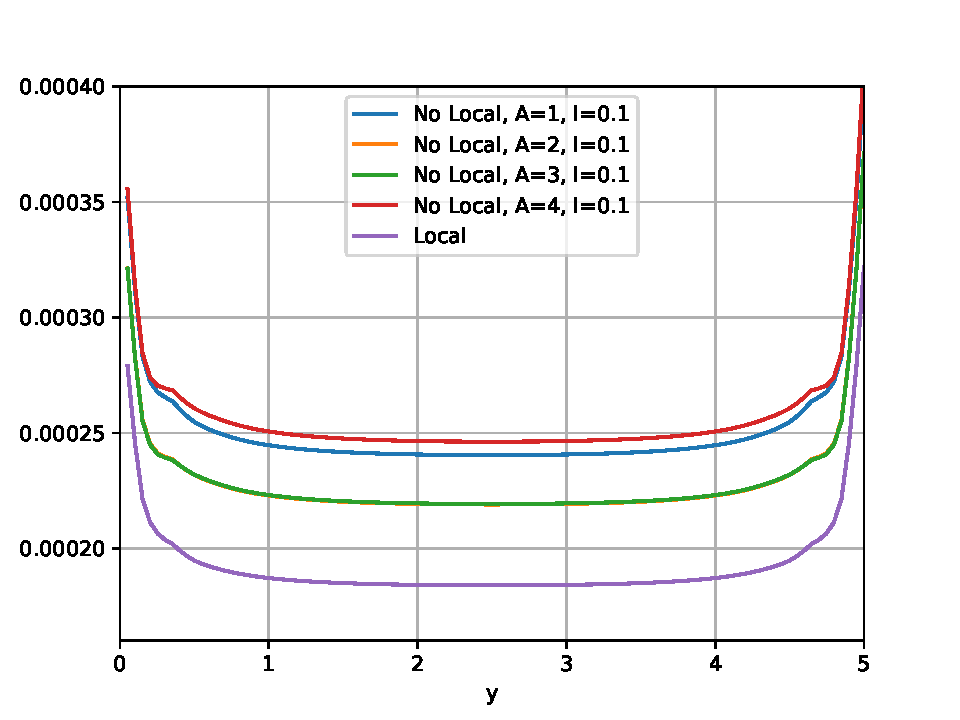
\includegraphics[width=\textwidth]{figuras/Placa/Perfiles/X/X0.1_0.019.pdf}
		        \caption{$l=0.1$}
		        \label{fig:perfilesX0019.01}
		    \end{subfigure}
		    \begin{subfigure}{0.48\textwidth}
		    \centering
		        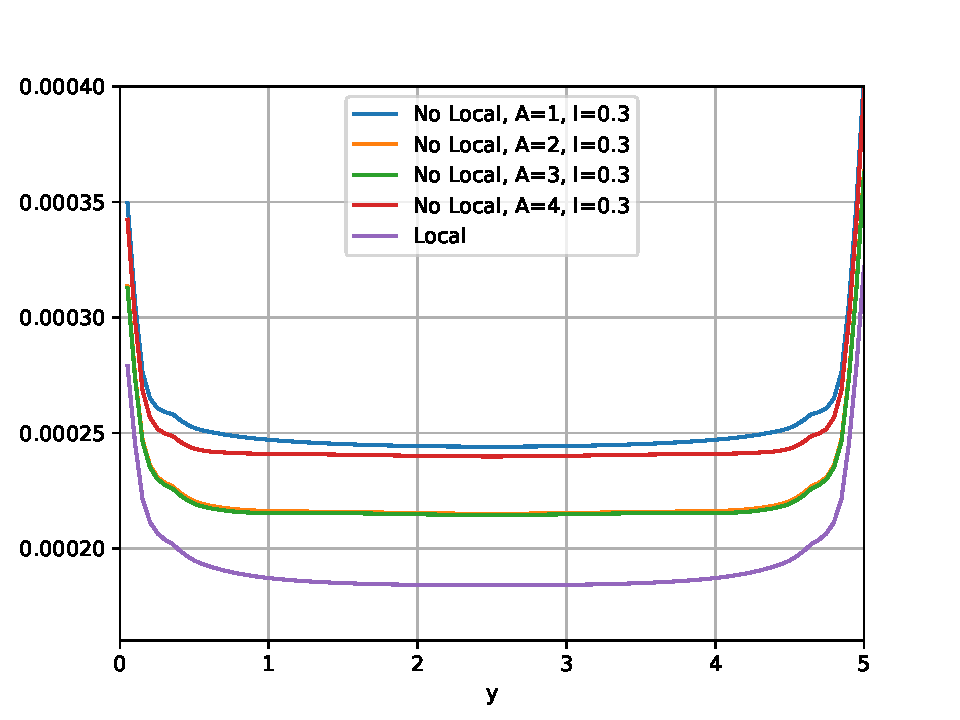
\includegraphics[width=\textwidth]{figuras/Placa/Perfiles/X/X0.3_0.019.pdf}
		        \caption{$l=0.3$}
		        \label{fig:perfilesX0019.03}
		    \end{subfigure}
		    \quad
		    \begin{subfigure}{0.48\textwidth}
		    \centering
		        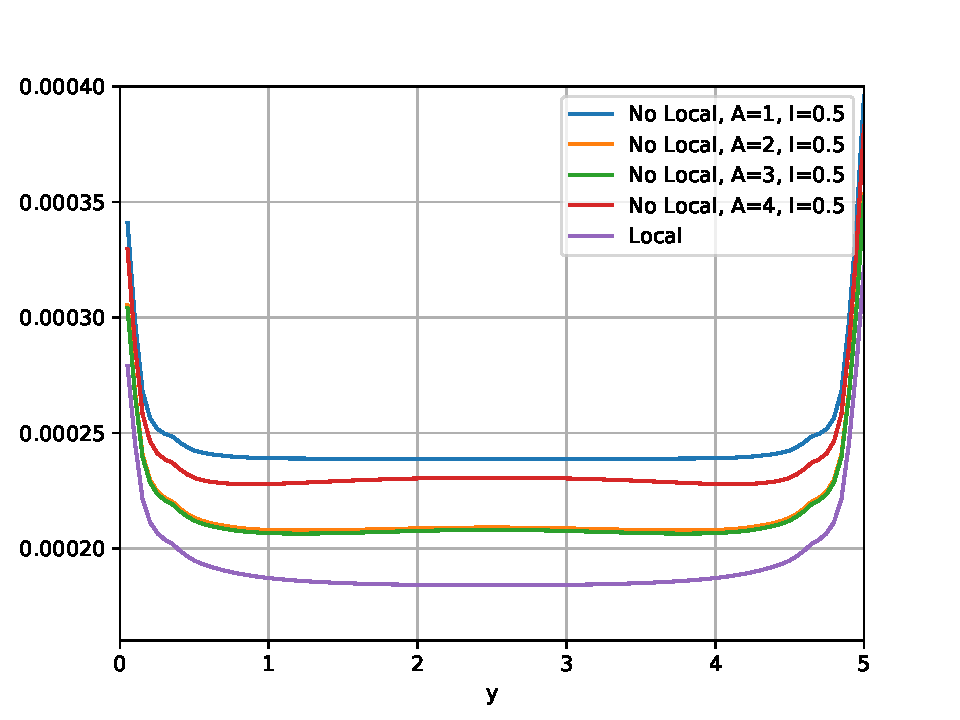
\includegraphics[width=\textwidth]{figuras/Placa/Perfiles/X/X0.5_0.019.pdf}
		        \caption{$l=0.5$}
		        \label{fig:perfilesX0019.05}
		    \end{subfigure}
		    \begin{subfigure}{0.48\textwidth}
		    \centering
		        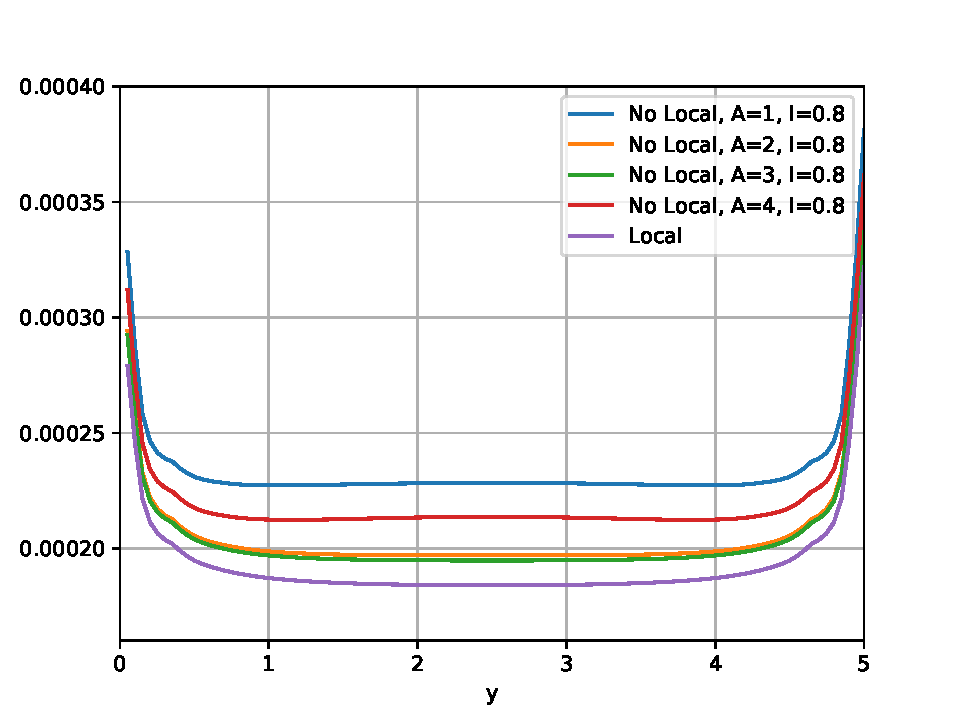
\includegraphics[width=\textwidth]{figuras/Placa/Perfiles/X/X0.8_0.019.pdf}
		        \caption{$l=0.8$}
		        \label{fig:perfilesX0019.08}
		    \end{subfigure}
		    \caption{Perfiles de $\varepsilon_x$ en $x=0.019$}
		    \label{fig:perfilesX0019}
		\end{figure}

	\subsubsection{\texorpdfstring{$x=2.519$}{x=2.519}}


		\begin{figure}
		    \centering
		    \sffamily
		    \begin{subfigure}{0.48\textwidth}
		    \centering
		        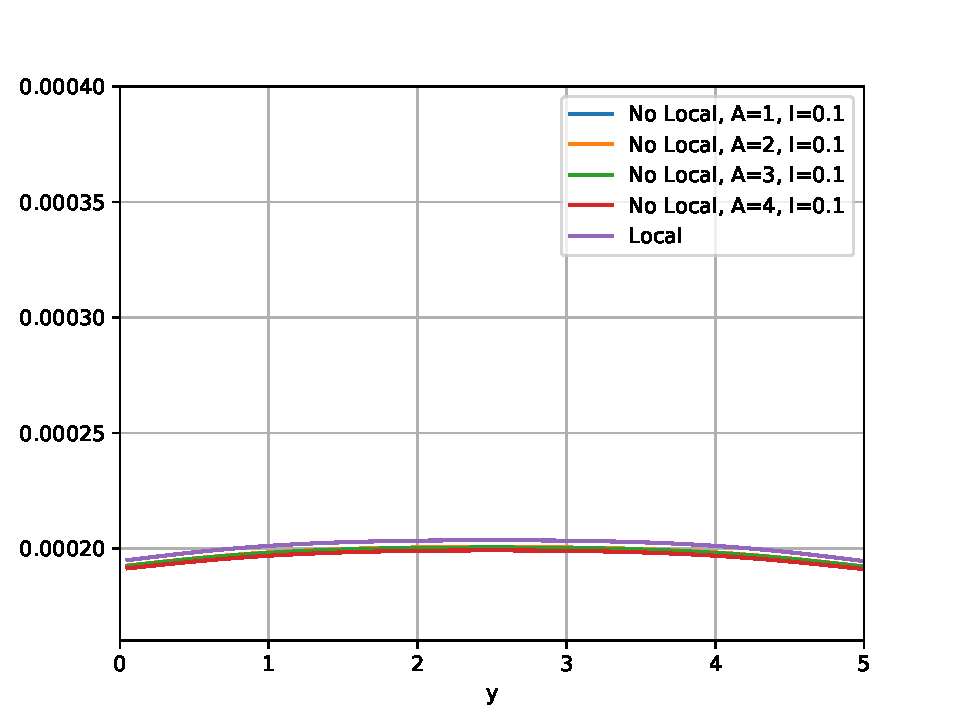
\includegraphics[width=\textwidth]{figuras/Placa/Perfiles/X/X0.1_2.519.pdf}
		        \caption{$l=0.1$}
		        \label{fig:perfilesX0259.01}
		    \end{subfigure}
		    \begin{subfigure}{0.48\textwidth}
		    \centering
		        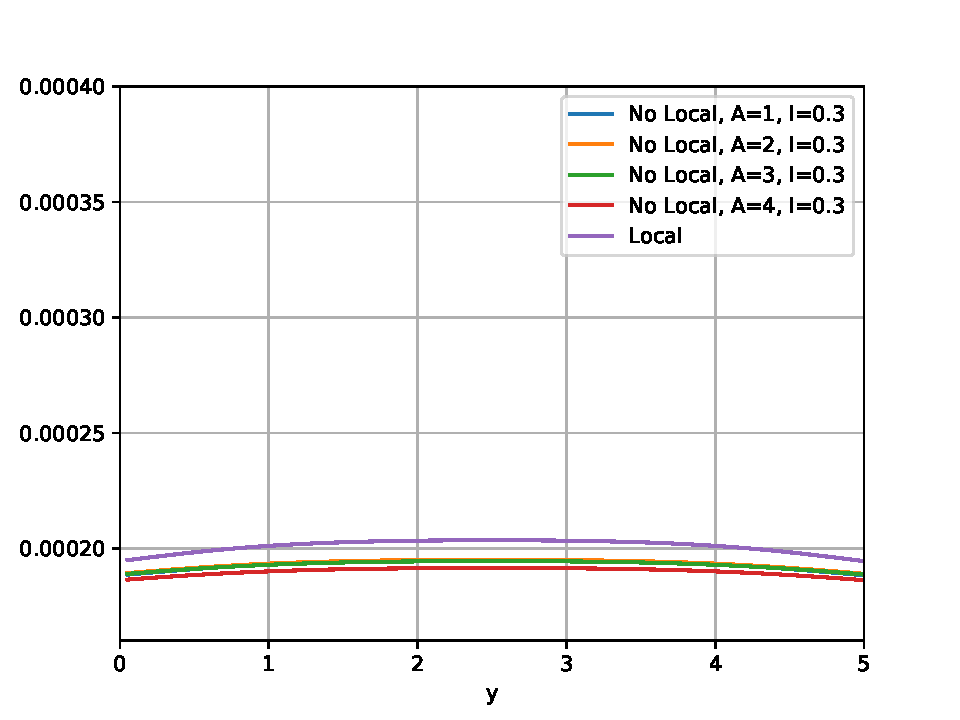
\includegraphics[width=\textwidth]{figuras/Placa/Perfiles/X/X0.3_2.519.pdf}
		        \caption{$l=0.3$}
		        \label{fig:perfilesX0259.03}
		    \end{subfigure}
		    \quad
		    \begin{subfigure}{0.48\textwidth}
		    \centering
		        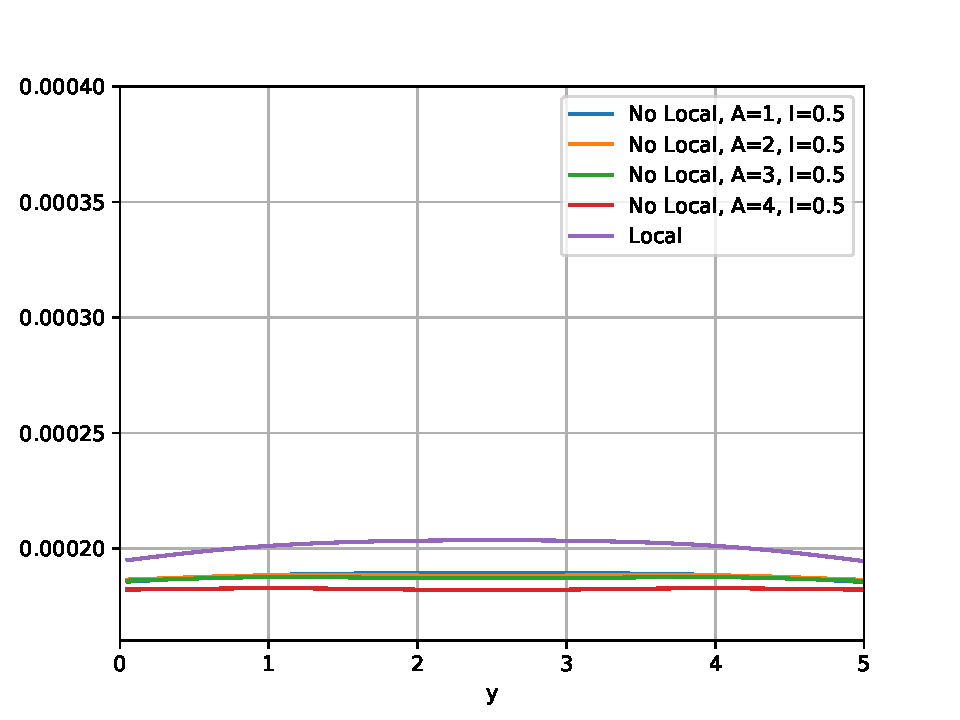
\includegraphics[width=\textwidth]{figuras/Placa/Perfiles/X/X0.5_2.519.pdf}
		        \caption{$l=0.5$}
		        \label{fig:perfilesX0259.05}
		    \end{subfigure}
		    \begin{subfigure}{0.48\textwidth}
		    \centering
		        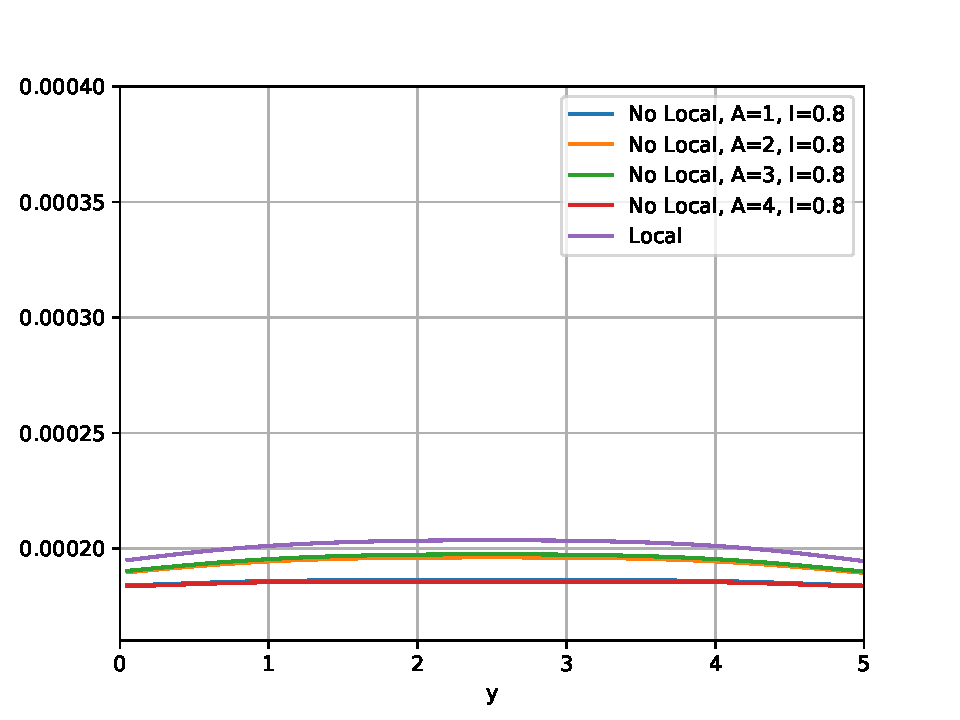
\includegraphics[width=\textwidth]{figuras/Placa/Perfiles/X/X0.8_2.519.pdf}
		        \caption{$l=0.8$}
		        \label{fig:perfilesX0259.08}
		    \end{subfigure}
		    \caption{Perfiles de $\varepsilon_x$ en $x=2.519$}
		    \label{fig:perfilesX0259}
		\end{figure}

	\subsubsection{\texorpdfstring{$y=0.019$}{y=0.019}}


		\begin{figure}
		    \centering
		    \sffamily
		    \begin{subfigure}{0.48\textwidth}
		    \centering
		        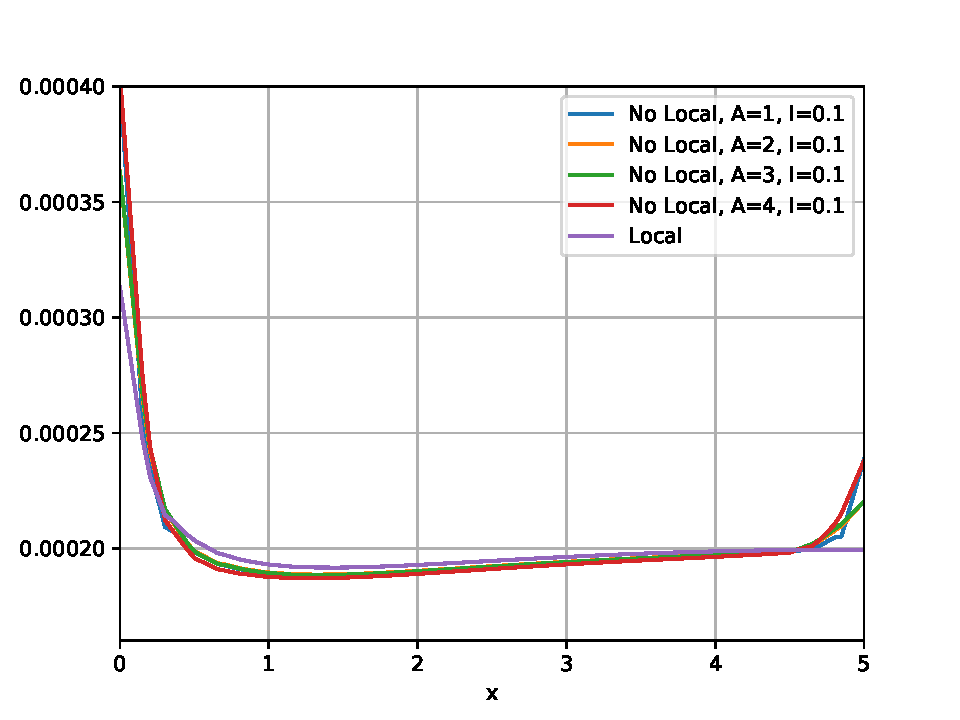
\includegraphics[width=\textwidth]{figuras/Placa/Perfiles/Y/Y0.1_0.019.pdf}
		        \caption{$l=0.1$}
		        \label{fig:perfilesY0019.01}
		    \end{subfigure}
		    \begin{subfigure}{0.48\textwidth}
		    \centering
		        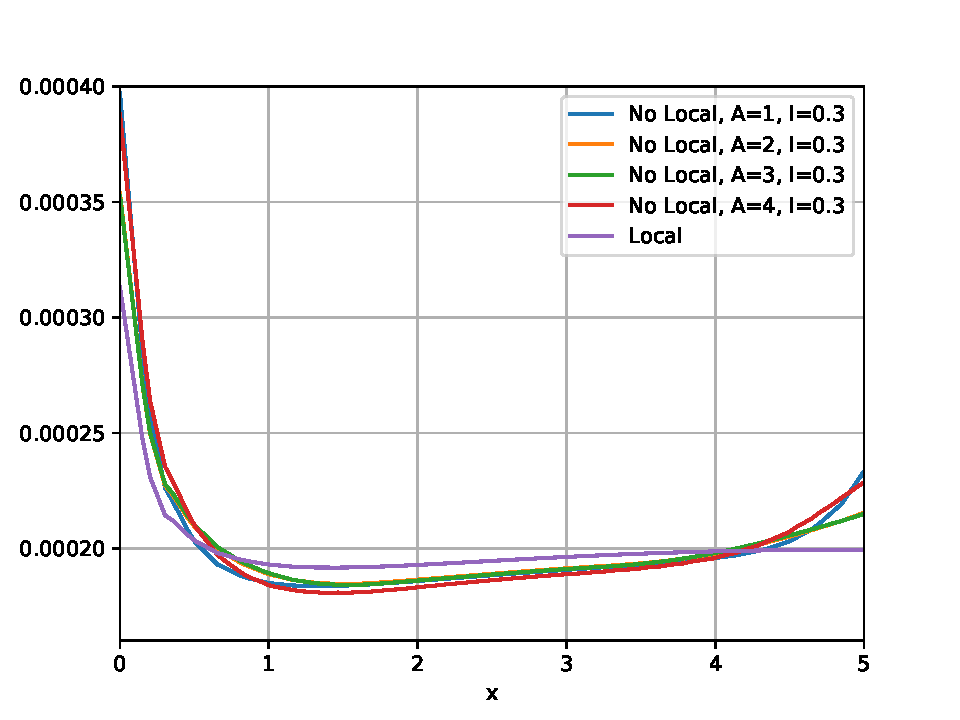
\includegraphics[width=\textwidth]{figuras/Placa/Perfiles/Y/Y0.3_0.019.pdf}
		        \caption{$l=0.3$}
		        \label{fig:perfilesY0019.03}
		    \end{subfigure}
		    \quad
		    \begin{subfigure}{0.48\textwidth}
		    \centering
		        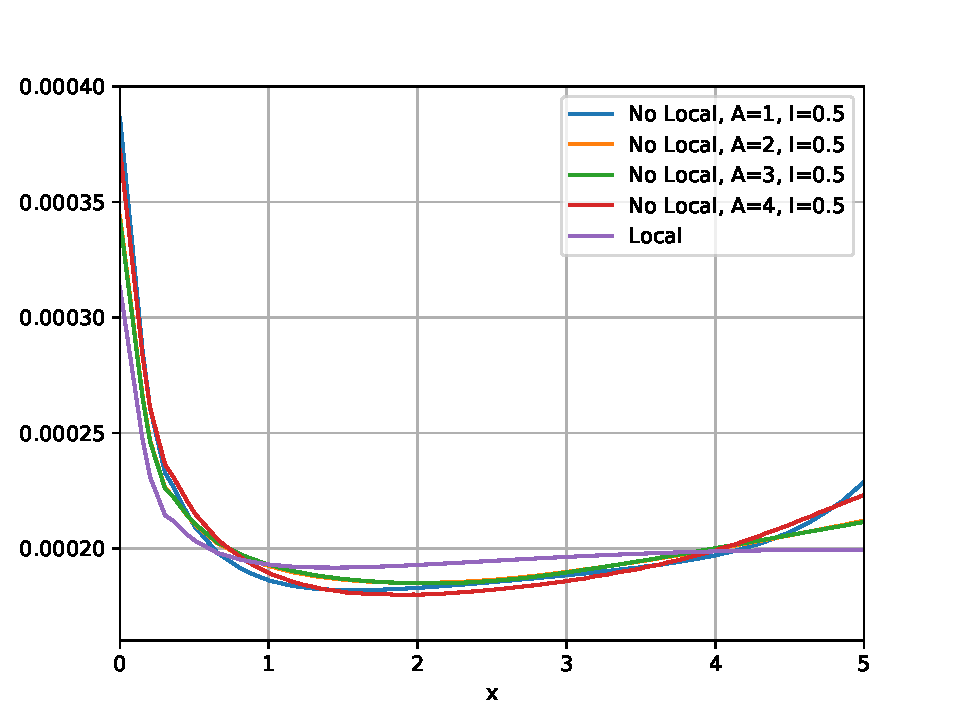
\includegraphics[width=\textwidth]{figuras/Placa/Perfiles/Y/Y0.5_0.019.pdf}
		        \caption{$l=0.5$}
		        \label{fig:perfilesY0019.05}
		    \end{subfigure}
		    \begin{subfigure}{0.48\textwidth}
		    \centering
		        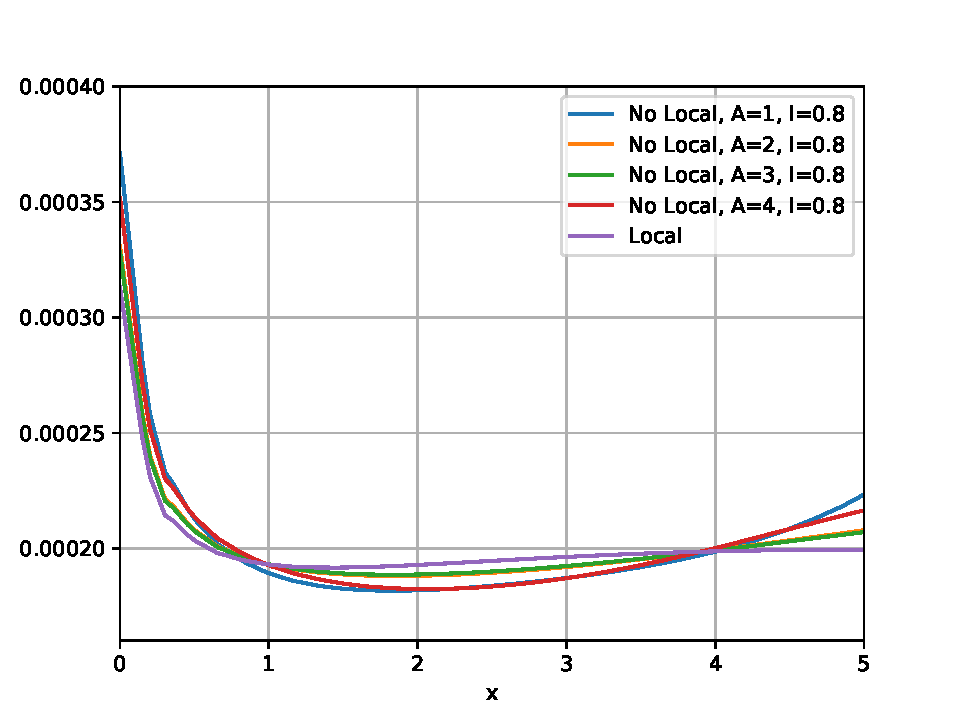
\includegraphics[width=\textwidth]{figuras/Placa/Perfiles/Y/Y0.8_0.019.pdf}
		        \caption{$l=0.8$}
		        \label{fig:perfilesY0019.08}
		    \end{subfigure}
		    \caption{Perfiles de $\varepsilon_x$ en $y=0.019$}
		    \label{fig:perfilesY0019}
		\end{figure}

	\subsubsection{\texorpdfstring{$y=2.519$}{y=2.519}}


		\begin{figure}
		    \centering
		    \sffamily
		    \begin{subfigure}{0.48\textwidth}
		    \centering
		        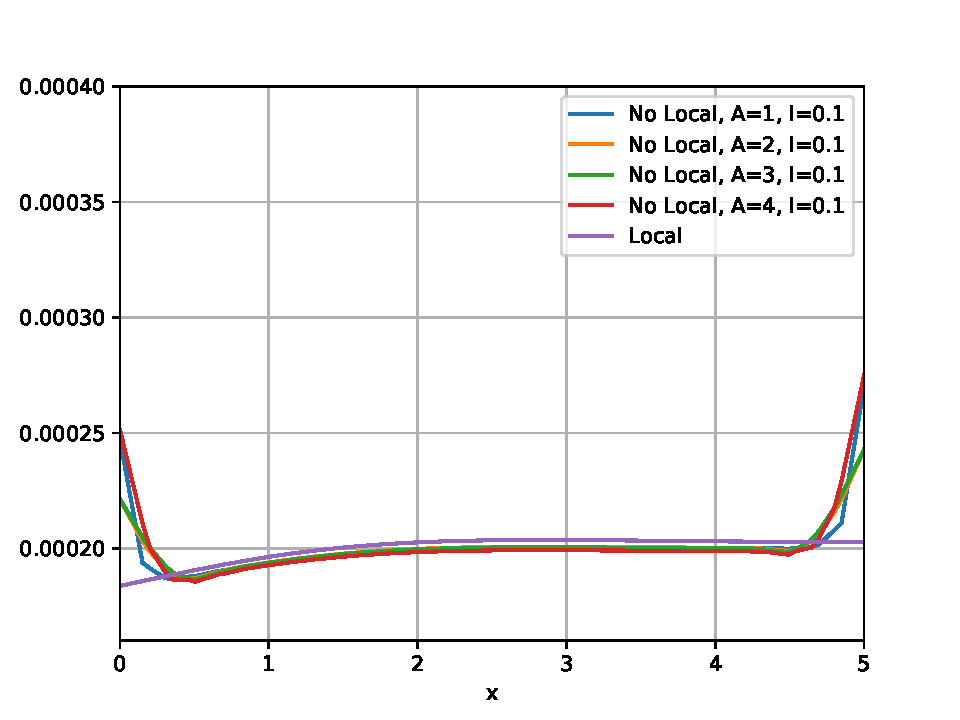
\includegraphics[width=\textwidth]{figuras/Placa/Perfiles/Y/Y0.1_2.519.pdf}
		        \caption{$l=0.1$}
		        \label{fig:perfilesY0259.01}
		    \end{subfigure}
		    \begin{subfigure}{0.48\textwidth}
		    \centering
		        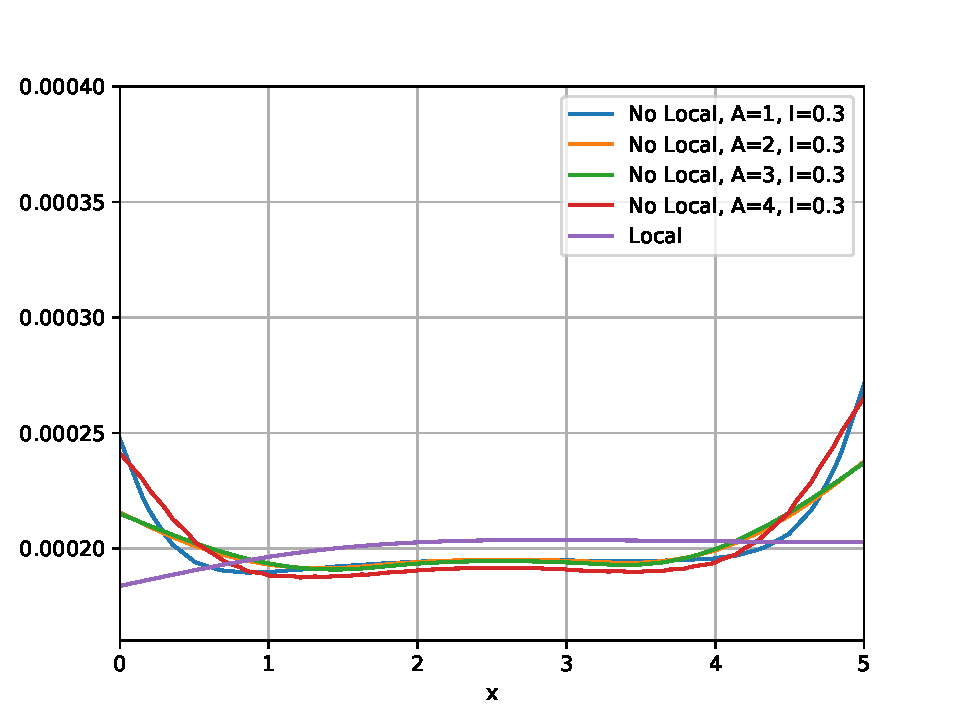
\includegraphics[width=\textwidth]{figuras/Placa/Perfiles/Y/Y0.3_2.519.pdf}
		        \caption{$l=0.3$}
		        \label{fig:perfilesY0259.03}
		    \end{subfigure}
		    \quad
		    \begin{subfigure}{0.48\textwidth}
		    \centering
		        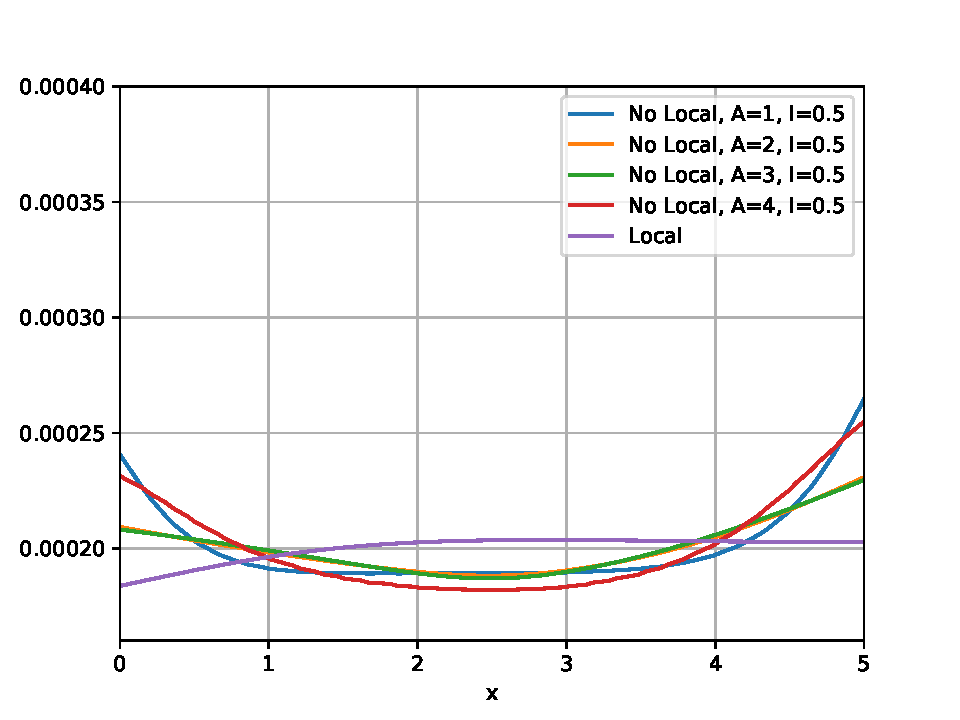
\includegraphics[width=\textwidth]{figuras/Placa/Perfiles/Y/Y0.5_2.519.pdf}
		        \caption{$l=0.5$}
		        \label{fig:perfilesY0259.05}
		    \end{subfigure}
		    \begin{subfigure}{0.48\textwidth}
		    \centering
		        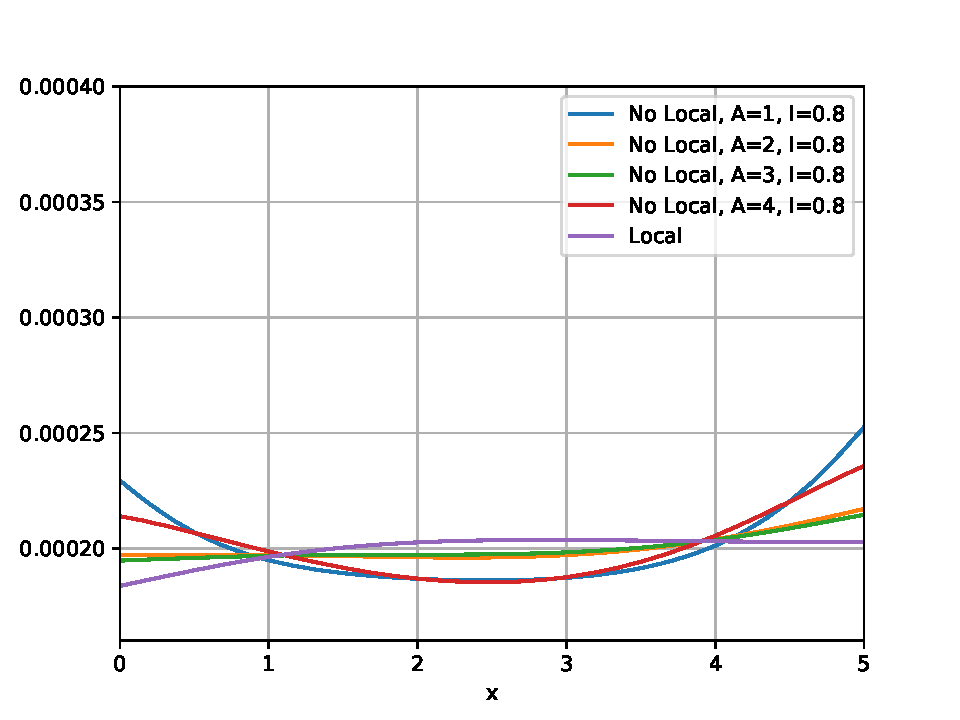
\includegraphics[width=\textwidth]{figuras/Placa/Perfiles/Y/Y0.8_2.519.pdf}
		        \caption{$l=0.8$}
		        \label{fig:perfilesY0259.08}
		    \end{subfigure}
		    \caption{Perfiles de $\varepsilon_x$ en $y=2.519$}
		    \label{fig:perfilesY0259}
		\end{figure}

\subsection{Caso de estudio 2: Barra a tensión}
	\subsubsection{\texorpdfstring{$x=0.125$}{y=0.125}}

		\begin{figure}
		    \centering
		    \sffamily
		    \begin{subfigure}{0.48\textwidth}
		    \centering
		        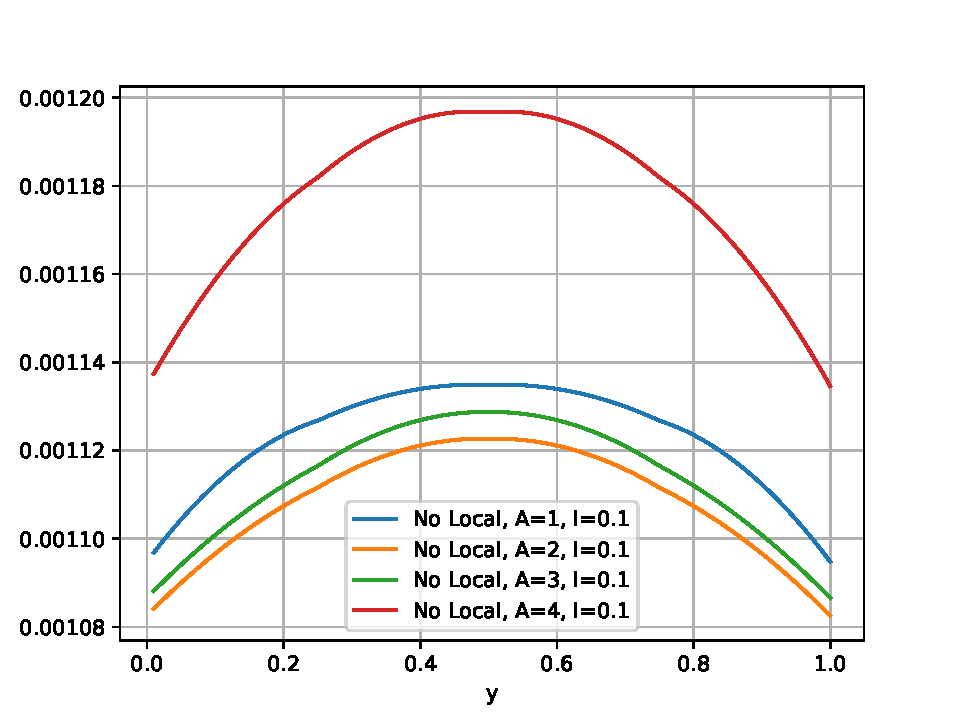
\includegraphics[width=\textwidth]{figuras/Barra/Perfiles/X/X0.1_0.125.pdf}
		        \caption{$l=0.1$}
		        \label{fig:perfilesbarraX0125.01}
		    \end{subfigure}
		    \begin{subfigure}{0.48\textwidth}
		    \centering
		        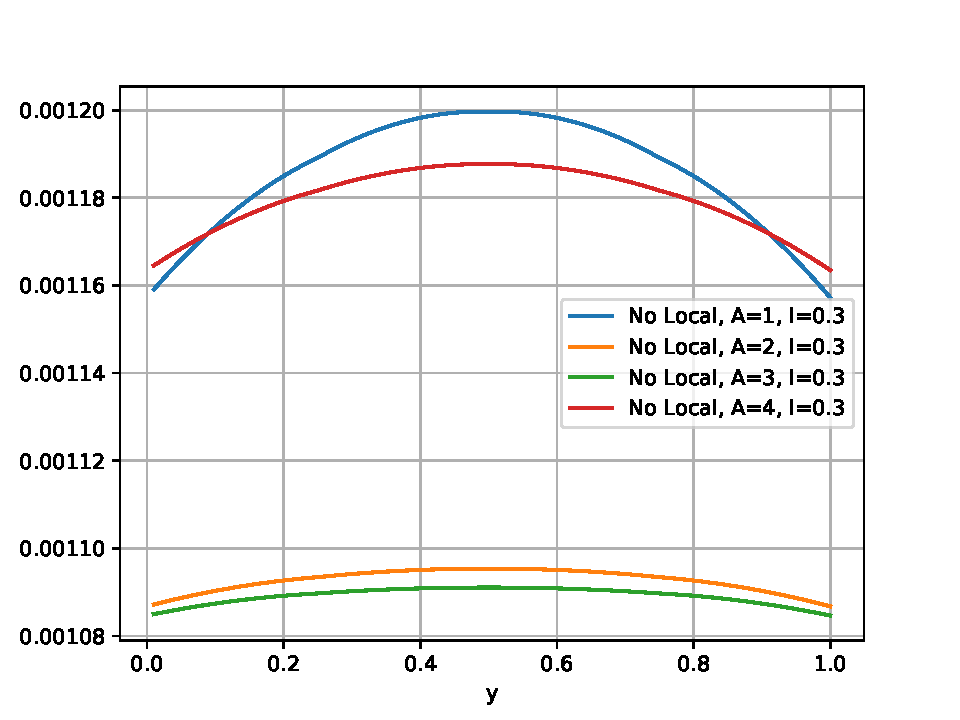
\includegraphics[width=\textwidth]{figuras/Barra/Perfiles/X/X0.3_0.125.pdf}
		        \caption{$l=0.3$}
		        \label{fig:perfilesbarraX0125.03}
		    \end{subfigure}
		    \quad
		    \begin{subfigure}{0.48\textwidth}
		    \centering
		        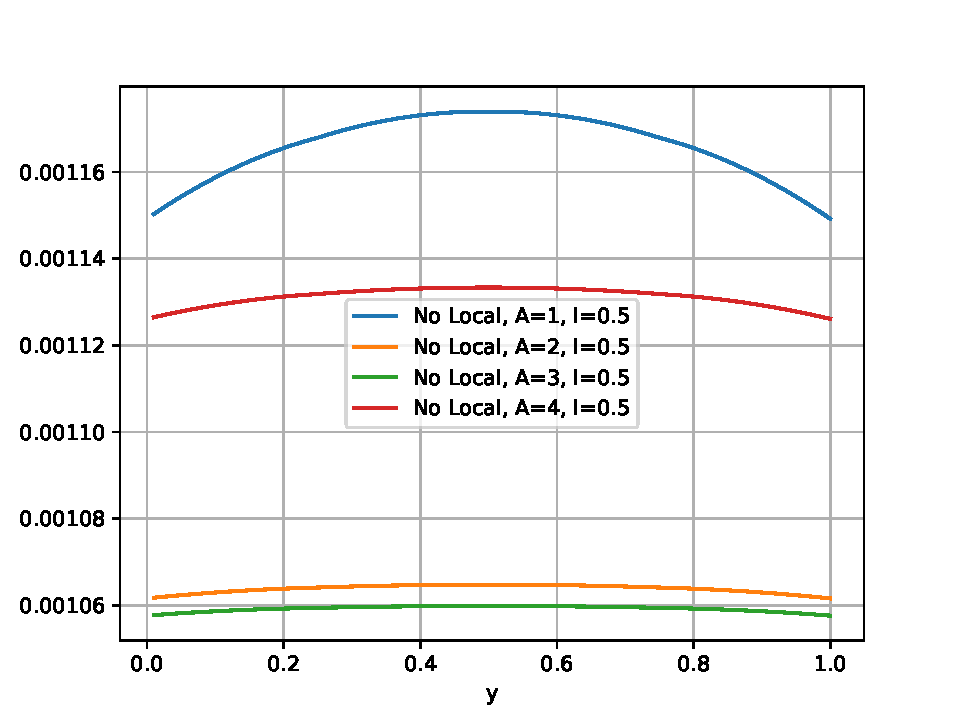
\includegraphics[width=\textwidth]{figuras/Barra/Perfiles/X/X0.5_0.125.pdf}
		        \caption{$l=0.5$}
		        \label{fig:perfilesbarraX0125.05}
		    \end{subfigure}
		    \begin{subfigure}{0.48\textwidth}
		    \centering
		        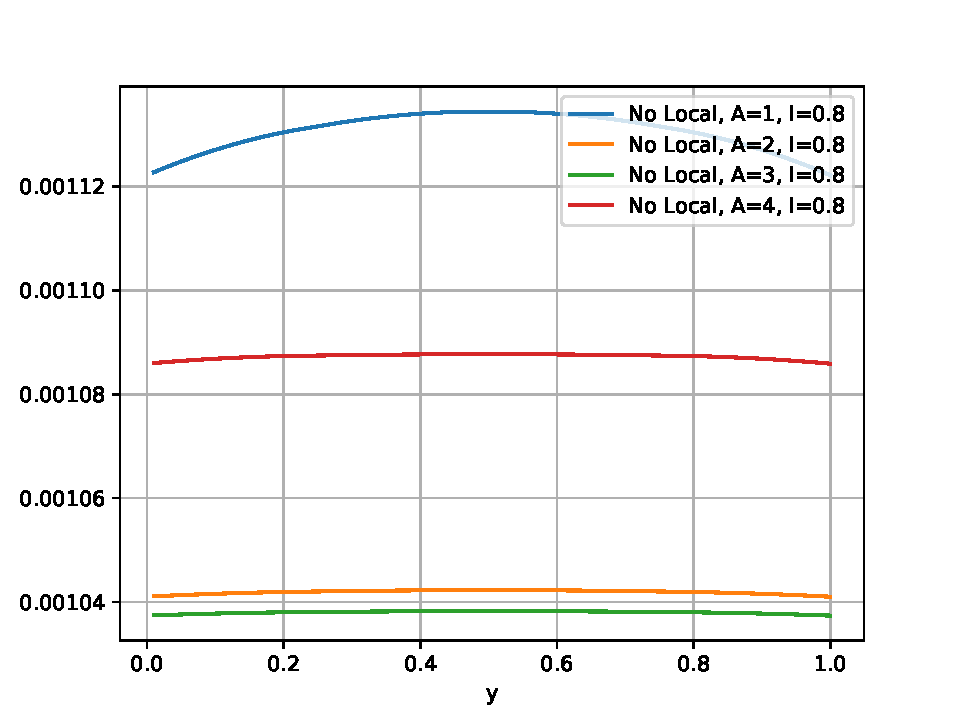
\includegraphics[width=\textwidth]{figuras/Barra/Perfiles/X/X0.8_0.125.pdf}
		        \caption{$l=0.8$}
		        \label{fig:perfilesbarraX0125.08}
		    \end{subfigure}
		    \caption{Perfiles de $\varepsilon_x$ en $x=0.125$}
		    \label{fig:perfilesbarraX0125}
		\end{figure}

	\subsubsection{\texorpdfstring{$y=0.472$}{y=0.472}}

		\begin{figure}
		    \centering
		    \sffamily
		    \begin{subfigure}{0.48\textwidth}
		    \centering
		        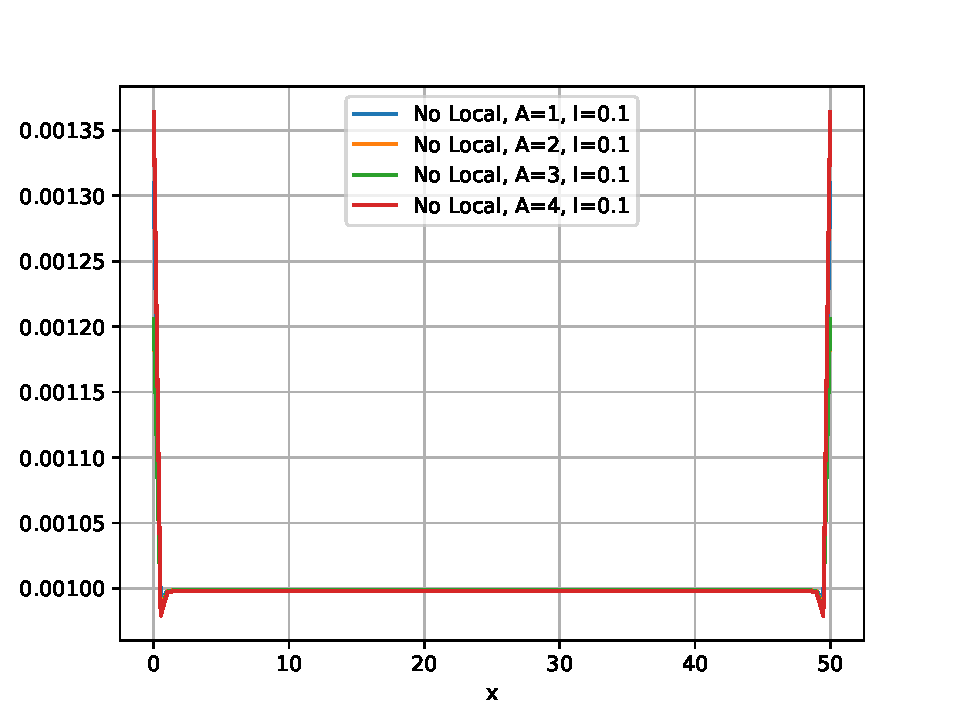
\includegraphics[width=\textwidth]{figuras/Barra/Perfiles/Y/Y0.1_0.472.pdf}
		        \caption{$l=0.1$}
		        \label{fig:perfilesbarraY0472.01}
		    \end{subfigure}
		    \begin{subfigure}{0.48\textwidth}
		    \centering
		        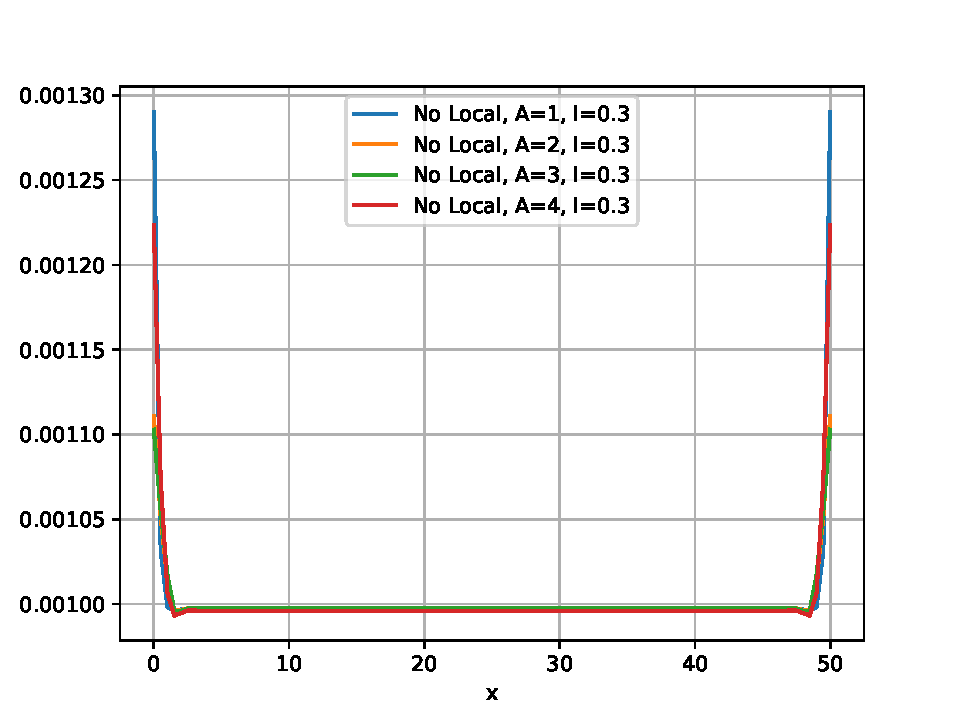
\includegraphics[width=\textwidth]{figuras/Barra/Perfiles/Y/Y0.3_0.472.pdf}
		        \caption{$l=0.3$}
		        \label{fig:perfilesbarraY0472.03}
		    \end{subfigure}
		    \quad
		    \begin{subfigure}{0.48\textwidth}
		    \centering
		        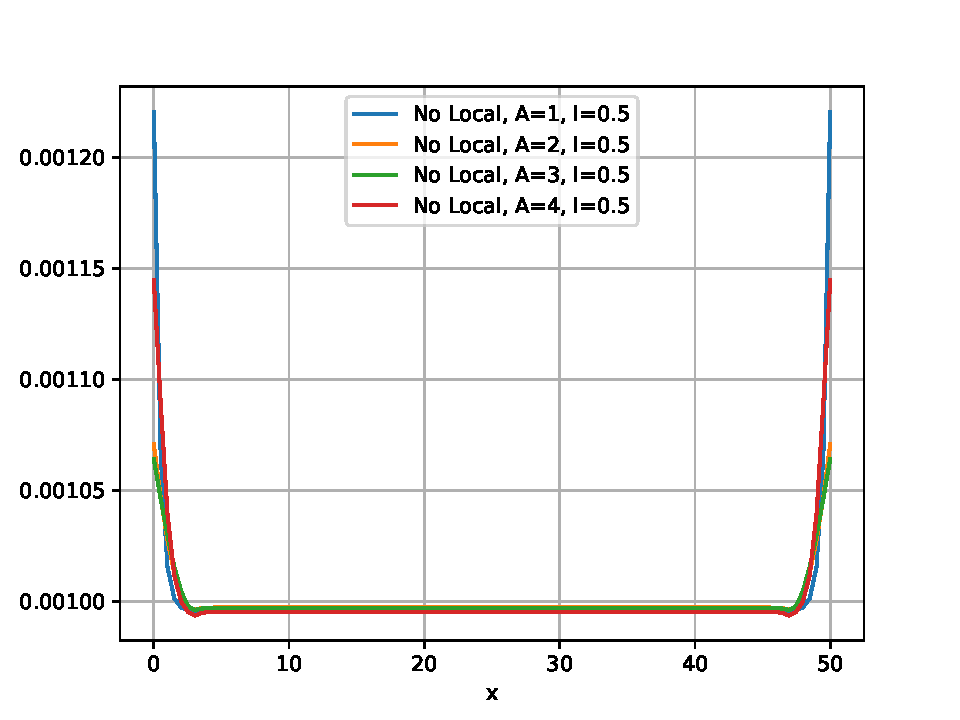
\includegraphics[width=\textwidth]{figuras/Barra/Perfiles/Y/Y0.5_0.472.pdf}
		        \caption{$l=0.5$}
		        \label{fig:perfilesbarraY0472.05}
		    \end{subfigure}
		    \begin{subfigure}{0.48\textwidth}
		    \centering
		        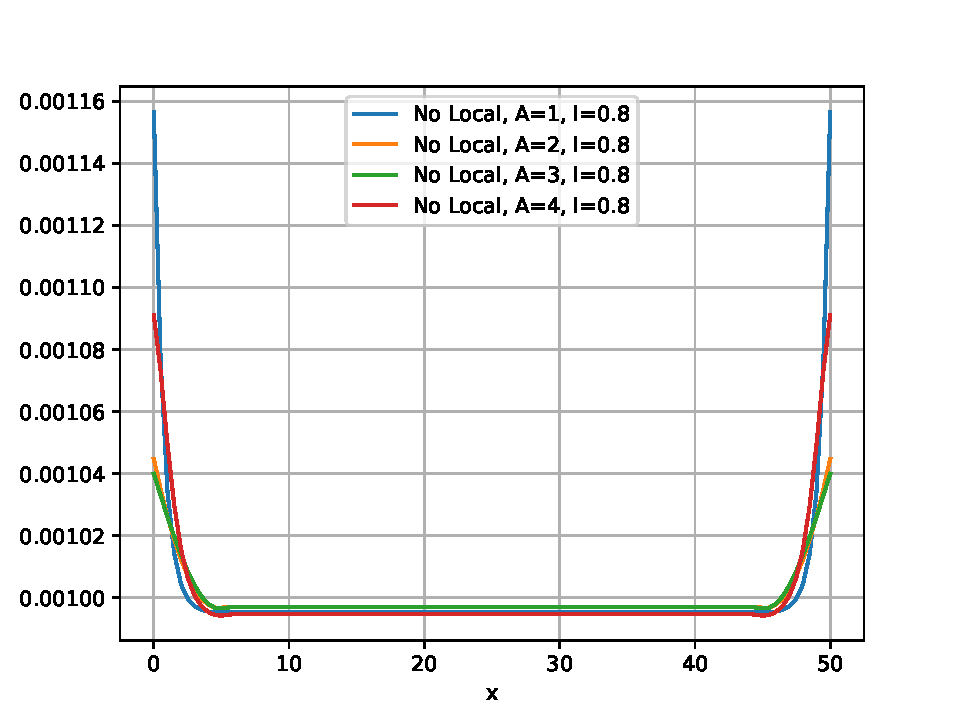
\includegraphics[width=\textwidth]{figuras/Barra/Perfiles/Y/Y0.8_0.472.pdf}
		        \caption{$l=0.8$}
		        \label{fig:perfilesbarraY0472.08}
		    \end{subfigure}
		    \caption{Perfiles de $\varepsilon_x$ en $y=0.472$}
		    \label{fig:perfilesbarraY0472}
		\end{figure}
